\documentclass[11pt]{article}
\usepackage{icmlko}
\begin{document}

\title{처음으로 안 본 도메인에 물어봤다 --- 전이가 0 이다}
\author{월드모델 실험실}
\date{노트 397 · 2026년 8월 2일}
\maketitle

\begin{abstract}
노트 380이 LODO 로 ``판은 새 도메인을 못 맞힌다''를 재고 남긴 유일한 직접
시험이 \emph{새 도메인 하나를 통째로 모아 예언과 대조}하는 것이었다.
열두 번째 도메인을 모았다 --- 애플 앱스토어 \textbf{비게임} 앱 1,600건
(21갈래 $\times$ 6목록, 2025년 이후 189건).

\textbf{자료가 한 건도 안 들어온 시점에 예측을 적었다}(노트 397 사전 등록):
$\rho = 0.4476 \pm 0.138$, 그리고 세 갈래 --- ㄱ 띠 안이면 노트 380 확인 ·
ㄴ 0 보다 크지만 띠 아래면 판이 과대평가 · \textbf{ㄷ 0 근처면 새 도메인에
전이가 없다}.

\textbf{설계의 핵심은 학습에 안 넣는 것이다.} F18 은 모르는 도메인에
원핫을 전부 0 으로 주므로 열한 도메인에서 배운 \emph{공유 계수만}으로
예측한다 --- 그것이 ``새 도메인 전이''의 정확한 정의다.

\begin{center}
\begin{tabular}{lrrr}
\hline
무리 & 행 & 모형 $\rho$ & 편상관(날짜 통제) \\
\hline
모바일 2025$+$ (\textbf{학습에 든 도메인}) & 441 & $+0.4801$ & $\mathbf{+0.4971}$ \\
앱 2025$+$ (\textbf{한 번도 안 본 도메인}) & 189 & $+0.2018$ & $\mathbf{+0.0824}$ \\
앱 전부 & 1,600 & $-0.0028$ & $\mathbf{-0.0021}$ \\
\hline
\end{tabular}
\end{center}
\emph{(둘 다 공유 축 다섯만 쓰게 맞췄다.)}

\textbf{6배다.} 그리고 1,600행 전체에서는 \textbf{0}이다($\pm0.025$).
189행에서 나온 $+0.082$ 도 $\pm0.073$ 이라 0 과 못 가른다.

\textbf{두 confound 를 다 막았다.} \emph{날짜} --- 앱 2025$+$ 에서는
달력 기준선이 $+0.4392$ 로 모형($+0.2273$)을 이긴다. 편상관으로 날짜를
빼면 모형이 $+0.1030$ 으로 내려앉는다. \emph{축} --- 앱은 공유 다섯만
있고 모바일은 트렌드 · 위키 · 달력을 더 갖는다. 모바일도 다섯만 쓰게
막으면 $+0.6026 \to +0.4971$ 로 18\% 주는데, \textbf{앱은 20\% 줄어
격차가 그대로다.} 격차는 축이 아니라 전이다.

\textbf{정직한 한계를 먼저 적는다.} 도메인이 하나이고, 비게임 앱은
생산성 · 금융 · 사진이 섞여 있어 \textbf{판의 열한 도메인이 다루는 ``IP
출시''가 아니다.} 공유 축 다섯(타깃 폭 · 장소 격 · 진입 마찰 · 매체 밀기 ·
굿즈 규모)이 유틸리티 앱에서 같은 뜻인지도 의심스럽다. \textbf{그래서 이
결과는 ``전이가 없다''의 첫 증거이지 마지막 증거가 아니다} --- 다음은
콘텐츠 도메인(팟캐스트)이다.
\end{abstract}

\section{왜 이 시험이 필요했나}

이 실험실의 판정치는 \emph{도메인마다 유보 $\rho$ 를 재고 표본 수로 가중
평균}한 것이다. 그 수가 0.45 라는 것은 ``우리가 가진 열한 도메인에서
평균적으로 이만큼 순위를 맞힌다''는 뜻이지 ``열두 번째에서도 그렇다''는
뜻이 아니다. \textbf{IP 파운데이션이라는 목표는 뒤엣것을 주장한다.}

노트 380이 LODO 로 그것을 간접적으로 쟀다 --- 도메인 하나를 빼고 나머지
열로 그 도메인을 맞히면 $|$오차$|$ 가 0.177 이고 도메인 $\rho$ 자체의
평균절대편차가 0.155 라, \textbf{중앙값을 부르는 것과 다를 바 없었다.}
그런데 LODO 는 여전히 \emph{학습에 그 도메인이 들어 있던} 모형의 점수를
쓴다. 진짜 시험은 한 번도 안 본 도메인이다.

\begin{figure}[t]
\centering
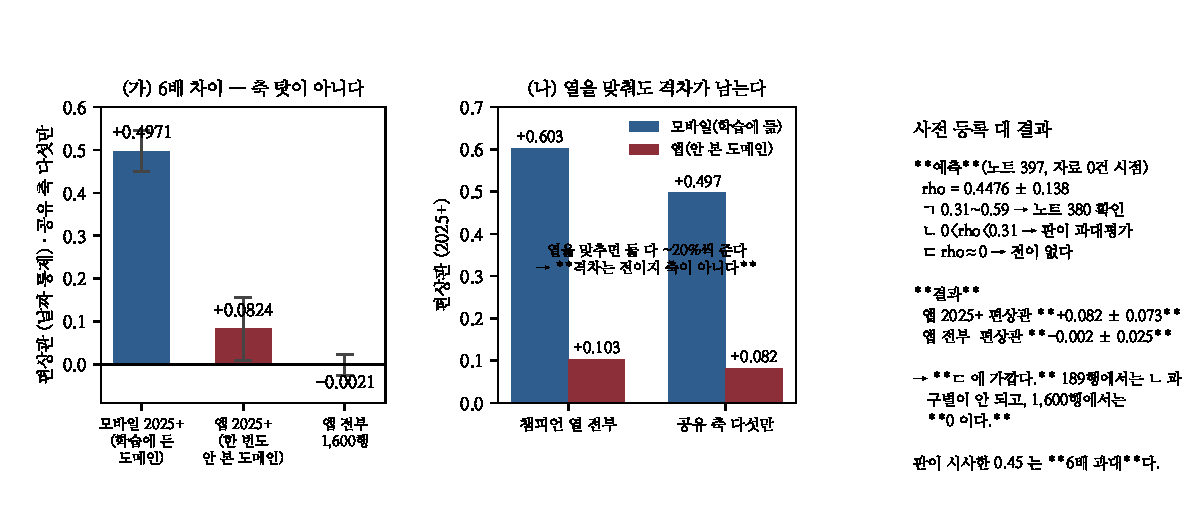
\includegraphics[width=\linewidth]{figs/fig397.pdf}
\caption{\textbf{(가)} 공유 축 다섯으로 맞춘 날짜 통제 편상관. 막대는
$1/\sqrt{n}$. \textbf{(나)} 열을 맞추기 전후 --- 둘 다 약 20\%씩 줄어
격차가 유지된다. \textbf{(다)} 사전 등록과 결과.}
\label{fig:main}
\end{figure}

\section{어떻게 모으고 어떻게 쟀나}

\textbf{도메인.} 애플 앱스토어 비게임 21갈래 $\times$ 6목록(인기 3 $+$
신규 3). 인기 목록만 쓰면 2025년 이후가 100개 중 16개뿐이라 신규 목록을
같이 훑었다. 출처 좌표(\texttt{\_genre} · 목록 출시일)를 남긴다(노트 383).

\textbf{라벨.} 평가 참여자 수 --- \textbf{모바일 게임과 같은 물리량}이다.
노트 377이 팝업에서 겪은 ``어느 자로 쟀나''를 안 만들려고 일부러 같은 자를
골랐다.

\textbf{축.} \texttt{ingest/mobile\_axes} 를 그대로 돌렸다. 다섯 축 덮음이
93\% 다.

\textbf{모형.} 챔피언 F18($K{=}32$)을 \textbf{열한 도메인 학습 행으로만}
적합하고 앱에 예측시켰다. 씨앗 여섯의 순위 평균을 쓴다(노트 395).

\section{결과 --- 세 겹으로 갈랐다}

\textbf{첫째, 날 것.} 앱 전부 $+0.1099$ · 앱 2025$+$ $+0.2273$. 사전 등록한
띠($0.31 \sim 0.59$) 아래다.

\textbf{둘째, 날짜.} 라벨이 누적 평가 수라 오래된 앱일수록 크다. 앱
2025$+$ 에서 달력 기준선($-$출시일)이 $\mathbf{+0.4392}$ 로 \textbf{모형을
이긴다.} 날짜를 빼는 편상관으로 보면 모형이 $+0.1030$ 이다. 네 구간에서
일관되게 $+0.10 \sim +0.16$ 이고 부호는 계속 양수다.

\textbf{셋째, 축.} 앱은 공유 다섯만 갖는데 모바일은 더 갖는다. \textbf{모바일도
다섯만 쓰게 막았다.}

\begin{center}
\begin{tabular}{lrr}
\hline
편상관(2025$+$) & 챔피언 열 전부 & 공유 다섯만 \\
\hline
모바일 (학습에 듦) & $+0.6026$ & $+0.4971$ \\
앱 (안 본 도메인) & $+0.1030$ & $+0.0824$ \\
\hline
비 & 5.9배 & \textbf{6.0배} \\
\hline
\end{tabular}
\end{center}

\textbf{열을 맞춰도 6배다.} 둘 다 18\,--\,20\% 씩 주므로 축의 차이는 격차를
설명하지 못한다.

\textbf{그리고 1,600행 전부에서는 $-0.0021 \pm 0.025$ 다} --- 0 이다.

\section{무엇을 주장하고 무엇을 안 주장하나}

\textbf{주장한다:} 이 판이 잰 0.45 는 \emph{새 도메인}에 대한 예언으로
쓰면 최소 6배 과대다. 한 번도 안 본 도메인에서 날짜를 통제하면 남는 것이
$+0.08$(189행, 0 과 구별 안 됨)이고 전체 1,600행에서는 0 이다.

\textbf{안 주장한다:} ``모형이 쓸모없다''고 안 한다. 학습에 든 도메인에서
$+0.50 \sim +0.60$ 은 실재하고 노트 387 · 393 · 394 가 그것이 자료에서
온다는 것을 위약으로 확인했다. \textbf{쓸모는 도메인 안에 있고, 도메인을
건너뛰지 못한다.}

\textbf{한계를 크게 적는다.} \emph{도메인이 하나다.} 그리고 비게임 앱은
생산성 · 금융 · 사진이 섞여 \textbf{IP 출시가 아니다} --- 공유 축 다섯이
그런 앱에서 같은 뜻인지 의심스럽고, 그렇다면 이 시험은 의도한 범위보다
\emph{어려운} 시험이다. \textbf{그래서 다음 도메인은 콘텐츠여야 한다} ---
팟캐스트(애플 차트, 같은 라벨 물리량, 명백한 IP)가 다음 후보다.

\section{남은 것}

\begin{center}
\begin{tabular}{lll}
\hline
항목 & 왜 값이 큰가 & 어떻게 \\
\hline
팟캐스트로 다시 & 비게임 앱은 IP 가 아니다 & 같은 절차, 같은 사전 등록 \\
콘텐츠 도메인 여럿 & 하나로는 못 정한다 & 세 개까지 늘려 분포를 본다 \\
전이가 어디서 죽나 & 축인가 계수인가 & 도메인 원핫을 켜고 껐을 때 차 \\
판정치를 고칠지 & 판이 전이를 시사하면 안 된다 & 표기에 ``학습 도메인 안'' 을 붙인다 \\
\hline
\end{tabular}
\end{center}

\end{document}
